\chapter{Dipoolstraling en verstrooiing}\label{ch:b2:dipole-radiation}

Waarom is de hemel blauw, en waarom is hij het blauwst haaks op de zon ---
en daar bovendien gepolariseerd, zoals bijen en fotografen weten? Waarom
moet een radiomast tientallen meters hoog zijn, en waarom straalt hij recht
omhoog niets uit? Beide vragen hebben hetzelfde antwoord: een trillende
elektrische lading straalt elektromagnetische golven uit, met een vermogen
dat als de vierde macht van de frequentie groeit en een patroon dat langs de
trillingsas verdwijnt. Dit hoofdstuk formuleert het veld van de
\emph{\omterm{thm:b2:dipole-radiation:field}{oscillerende dipool}}, het eenvoudigste stralende stelsel, leidt
daaruit de antenne en de straling van een versnelde lading af, en past het
toe op de moleculen van de lucht, die elk een minuscule antenne zijn die het
zonlicht opnieuw uitzendt: \omterm{prop:b2:dipole-radiation:rayleigh}{rayleighverstrooiing}.

\begin{omfigure}
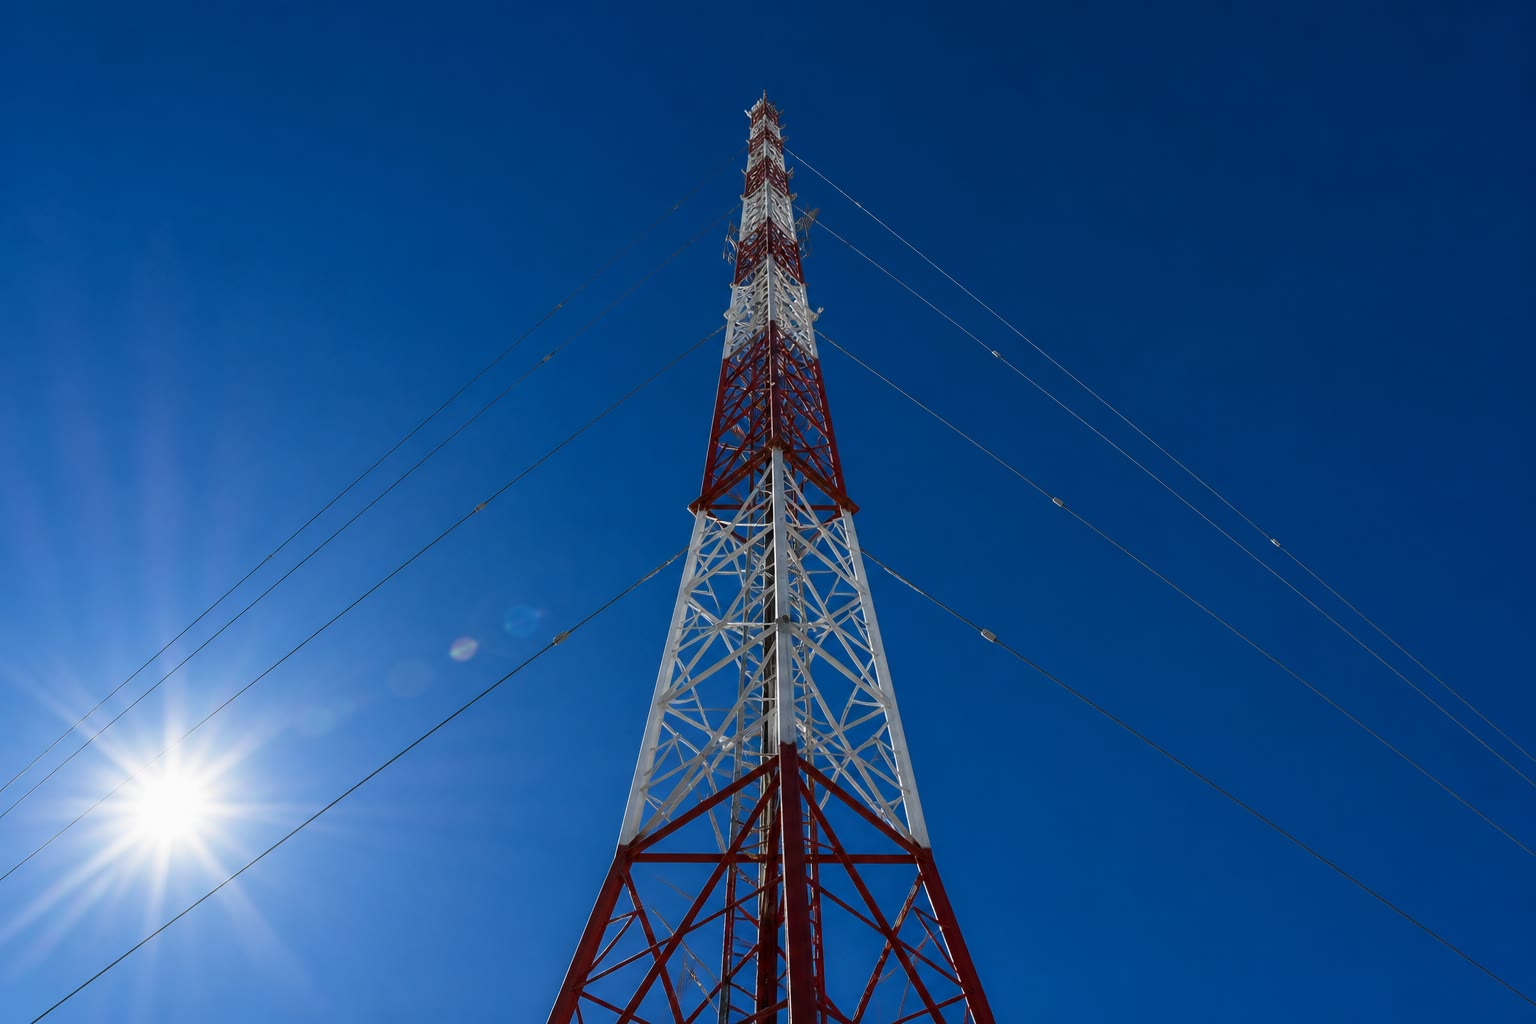
\includegraphics[width=0.54\linewidth]{images/book4/ai/b4-17-radio-mast-blue-sky.jpg}

{\small Een zendmast onder een blauwe hemel: een verticale dipool van
tientallen meters die naar de horizon straalt, en daarboven de hemel die
door miljarden moleculaire dipolen wordt verlicht die de zon opnieuw
uitstralen.}
\end{omfigure}


\section{Het veld van een oscillerende dipool}

\begin{theorem}[Stralingsveld van een elektrische dipool]\label{thm:b2:dipole-radiation:field}
\index{oscillerende dipool}\index{stralingszone}\index{vertraging (retardatie)}
Een dipool met moment $\vect p(t) = p_0\cos\omega t\,\vect e_z$ en afmeting
$a$, in de oorsprong, straalt. In de \emph{stralingszone} --- op afstanden
$r \gg
\lambda = 2\pi c/\omega \gg a$ --- is zijn veld, in bolcoördinaten
$(r,
\theta, \varphi)$ om de as van de dipool,
\[
\vect E(M, t) = -\frac{\mu_0\,\omega^2p_0}{4\pi}\,\frac{\sin\theta}r\,\cos\bigl(\omega(t - r/c)\bigr)\,\vect e_\theta ,
\qquad
\vect B = \frac{\vect e_r\wedge\vect E}c :
\]
een \omterm{prop:b2:sound-waves:spherical}{bolgolf} die plaatselijk vlak is --- $(\vect E, \vect B, \vect e_r)$ een
rechtsdraaiend drietal met $B = E/c$ --- \emph{vertraagd} met de looptijd
$r/c$, met een amplitude die als $1/r$ daalt, evenredig met de versnelling
$\ddot p = -\omega^2p$ van de dipool en met $\sin\theta$: maximaal in het
equatorvlak, nul langs de as; gepolariseerd in het vlak dat de as bevat.
\end{theorem}
\admitted

\begin{remark}[De formule lezen]\label{rem:b2:dipole-radiation:reading}
De exacte oplossing van de \omterm{thm:b2:maxwell-equations:maxwell}{vergelijkingen van Maxwell} (uit de vertraagde
potentialen, buiten het bereik van dit volume) bevat ook termen in $1/r^2$
en $1/r^3$; de laatste is het quasistatische dipoolveld van het volume van
jaar 1, $\vect E \propto p/4\pi\varepsilon_0r^3$, dat in de
\emph{nabijheidszone} $r \ll \lambda$ overheerst; bij $r \sim \lambda/2\pi$
zijn de twee vergelijkbaar, en daarvoorbij overleeft alleen de term in
$1/r$. Elke factor heeft een reden. $1/r$: het vermogen door een bol,
$\propto E^2r^2$, mag niet van $r$ afhangen. $\omega^2p_0$: het veld van een
lading in rust of in eenparige beweging straalt niet; het is de
\emph{versnelling} die straalt. $\sin\theta$: een waarnemer op de as ziet de
lading langs zijn zichtlijn heen en weer gaan, zonder transversale
versnelling; in het equatorvlak is de hele versnelling transversaal.
Vertraging: het veld in $M$ op het tijdstip $t$ weerspiegelt wat de dipool
op $t - r/c$ deed.
\end{remark}

\begin{omfigure}
\begin{tikzpicture}[font=\small, x=1cm, y=1cm, >=Stealth]
  \begin{scope}
    \draw[->, thick] (0,-2.2) -- (0,2.4) node[right, font=\footnotesize] {$z$};
    \draw[omThm, very thick, <->] (0,-0.5) -- (0,0.5); \node[omThm, font=\footnotesize] at (0.35,0.0) {$\vect p$};
    \coordinate (M) at (2.6,1.6);
    \draw[dashed] (0,0) -- (M); \fill (M) circle (1.5pt); \node[font=\footnotesize] at (2.45,1.25) {$M$};
    \draw (0,0.7) arc[start angle=90, end angle=31.6, radius=0.7]; \node[font=\footnotesize] at (0.35,0.9) {$\theta$};
    \draw[omDef, very thick, ->] (M) -- ($(M)+(0.55,-0.9)$) node[right, font=\footnotesize] {$\vect E$ ($\vect e_\theta$)};
    \node[omProp, font=\footnotesize] at ($(M)+(-0.65,0.25)$) {$\vect B$ $\otimes$};
    \draw[omExo, thick, ->] (M) -- ($(M)+(0.7,0.43)$) node[right, font=\footnotesize] {$\vect e_r$};
    \node[font=\footnotesize] at (0,-2.7) {$E \propto \dfrac{\omega^2p_0\sin\theta}{r}\cos\omega(t - r/c)$};
  \end{scope}
  \begin{scope}[xshift=8.6cm]
    \draw[->, thick] (0,-2.2) -- (0,2.4) node[right, font=\footnotesize] {$z$};
    \draw[omThm, thick, domain=0:360, samples=120, smooth] plot ({2.0*sin(\x)*sin(\x)*sin(\x)},{2.0*sin(\x)*sin(\x)*cos(\x)});
    \draw[omThm, very thick, <->] (0,-0.35) -- (0,0.35);
    \node[omThm, font=\footnotesize] at (2.3,0.35) {$\sin^2\theta$};
    \node[font=\footnotesize] at (0,-2.7) {uitgestraald vermogen per ruimtehoek};
  \end{scope}
\end{tikzpicture}

{\small Links: het stralingsveld van een dipool in een ver punt $M$ ---
transversaal, langs $\vect e_\theta$, met een azimutale $\vect B$; langs de
as wordt niets uitgestraald. Rechts: het stralingsdiagram, een torus
$\propto\sin^2\theta$ waarvan de doorsnede is getekend.}
\end{omfigure}

\section{Uitgestraald vermogen}

\begin{proposition}[Vermogen van een dipool; formule van Larmor]\label{prop:b2:dipole-radiation:power}
\index{uitgestraald vermogen (dipool)}\index{formule van Larmor}\index{stralingsdiagram}
De gemiddelde \omterm{thm:b2:poynting-vector:poynting}{poyntingvector} van het veld van de dipool is radiaal,
\[
\langle\vect\Pi\rangle = \frac{\mu_0\,\omega^4p_0^2}{32\pi^2c}\,\frac{\sin^2\theta}{r^2}\,\vect e_r ,
\]
en het totale gemiddelde uitgestraalde vermogen is
\[
\mathcal P = \frac{\mu_0\,\omega^4p_0^2}{12\pi c} = \frac{p_0^2\omega^4}{12\pi\varepsilon_0c^3} .
\]
Voor één enkele lading $q$ met versnelling $a$ (niet-relativistisch) is het
ogenblikkelijke vermogen $\mathcal P = q^2a^2/6\pi\varepsilon_0c^3$
(Larmor).
\end{proposition}

\begin{proof}
$\langle\Pi\rangle = \langle E^2\rangle/\mu_0c$ met
$\langle\cos^2\rangle = \tfrac12$; integreer over de bol:
\[
\int\sin^2\theta\,r^2\dd\Omega = 2\pi r^2\int_0^\pi\sin^3\theta\,\dd\theta = \tfrac83\pi r^2 ,
\qquad
\mathcal P = \frac{\mu_0\omega^4p_0^2}{32\pi^2c}\cdot\frac{8\pi}3 = \frac{\mu_0\omega^4p_0^2}{12\pi c} .
\]
Larmor: $p = qz$, dus $\ddot p = qa$; het gemiddelde
$\tfrac12\omega^4p_0^2 = \langle\ddot p^2\rangle$ vervangen door het
ogenblikkelijke $q^2a^2$ geeft $\mathcal P = \mu_0q^2a^2/6\pi c$.
\end{proof}

\begin{example}[Een antenne en een draad]\label{ex:b2:dipole-radiation:antenna}
\index{antenne}\index{stralingsweerstand}\index{halvegolfdipool}
Een korte draad met lengte $\ell \ll \lambda$ die de stroom
$I_0\cos\omega t$ voert, is een dipool met $\dot p = I_0\ell\cos\omega t$,
dus $p_0 = I_0\ell/\omega$: hij straalt
$\mathcal P = \mu_0\omega^2I_0^2\ell^2/12\pi c = \tfrac12R_{\text{str}}I_0^2$
uit, met de \emph{\omterm{ex:b2:dipole-radiation:antenna}{stralingsweerstand}}
$R_{\text{str}} = \dfrac{2\pi}3\sqrt{\dfrac{\mu_0}{\varepsilon_0}}
\Bigl(\dfrac\ell\lambda\Bigr)^2 \approx 790\,(\ell/\lambda)^2\ \Omega$
--- het vermogen verlaat de kring alsof het door een weerstand gaat, zonder
dat er iets warm wordt. Een draad van \qty{1}{m} bij \qty{1}{MHz}
($\lambda = \qty{300}{m}$): $R_{\text{str}} = \qty{9}{m\ohm}$, minder dan
zijn koperweerstand, een slechte antenne; bij \qty{100}{MHz}: \qty{88}{\ohm}
(de formule voor een korte dipool wordt hier opgerekt), een goede. De
\emph{\omterm{ex:b2:dipole-radiation:antenna}{halvegolfdipool}}, $\ell = \lambda/2$ met een sinusvormige
stroomverdeling, heeft $R_{\text{str}} = \qty{73}{\ohm}$ (aangenomen) en een
diagram dat dicht bij dat van de elementaire dipool ligt --- de
standaardantenne, van zendmasten tot de sprietantennes op oude televisies.
Een netdraad van \qty{1}{m} bij \qty{50}{Hz}:
$R_{\text{str}} \approx \qty{2e-11}{\ohm}$ --- de quasistationaire
schakelingen van \cref{ch:b2:maxwell-equations} stralen niets uit.
\end{example}

\begin{omfigure}
\begin{tikzpicture}[font=\small, x=1cm, y=1cm, >=Stealth]
  \begin{scope}
    \draw[thick] (-2.4,0) -- (-0.15,0); \draw[thick] (0.15,0) -- (2.4,0);
    \draw[omExo, thick] (-0.15,0) -- (-0.15,-0.6) (0.15,0) -- (0.15,-0.6);
    \node[omExo, font=\footnotesize] at (0,-0.9) {voeding};
    \draw[omThm, thick, domain=-2.4:2.4, samples=60] plot (\x,{1.0*cos(deg(pi*\x/4.8))});
    \foreach \x in {-2.0,-1.2,-0.4,0.4,1.2,2.0} \draw[omThm, ->] (\x,0) -- (\x,{1.0*cos(deg(pi*\x/4.8))});
    \node[omThm, font=\footnotesize] at (1.5,1.25) {$I(z)$};
    \draw[<->] (-2.4,-1.3) -- (2.4,-1.3) node[midway, below, font=\footnotesize] {$\lambda/2$};
    \node[font=\footnotesize] at (0,-2.2) {halvegolfdipool: $R_{\text{str}} = \qty{73}{\ohm}$};
  \end{scope}
  \begin{scope}[xshift=8.0cm]
    \begin{axis}[omaxis, axis x line=bottom, axis y line=left, width=5.6cm, height=4.2cm, at={(0,-1.9cm)},
        xmode=log, ymode=log, xmin=1e-3, xmax=0.5, ymin=1e-3, ymax=300,
        xlabel={$\ell/\lambda$}, ylabel={$R_{\text{str}}$ ($\Omega$)}, xtick={1e-3,1e-2,1e-1}, ytick={1e-3,1e-1,10},
        xlabel style={at={(axis description cs:0.5,-0.12)}, anchor=north},
        ylabel style={at={(axis description cs:-0.2,0.5)}, rotate=90, anchor=south}, samples=40]
      \addplot[omDef, thick, domain=1e-3:0.3] {790*x*x};
      \addplot[only marks, mark=*, mark size=1.8pt, omThm] coordinates {(0.5,73)};
    \end{axis}
  \end{scope}
\end{tikzpicture}

{\small Links: de stroomverdeling op een \omterm{ex:b2:dipole-radiation:antenna}{halvegolfdipool}, maximaal bij de
voeding en nul aan de uiteinden. Rechts: de \omterm{ex:b2:dipole-radiation:antenna}{stralingsweerstand} van een korte
dipool, $790(\ell/\lambda)^2$ ohm, en de \qty{73}{\ohm} van de
\omterm{ex:b2:dipole-radiation:antenna}{halvegolfdipool}.}
\end{omfigure}

\begin{example}[Een elektron dat straalt]\label{ex:b2:dipole-radiation:electron}
In een röntgenbuis wordt een elektron van \qty{50}{keV}
($v = \qty{1.2e8}{m/s}$) in \qty{1}{\micro m} wolfraam gestopt:
$a \sim v^2/2d = \qty{7e21}{m/s^2}$, vermogen volgens Larmor
$\qty{1.2e-4}{W}$ gedurende $\qty{1.6e-14}{s}$: \qty{2e-18}{J}, ongeveer
$0.02\%$ van zijn energie uitgestraald als de ``remstraling'' van de buis
--- de rest is warmte, en de anode wordt gekoeld. Het klassieke elektron van
een waterstofatoom, met een versnelling $v^2/r = \qty{9e22}{m/s^2}$, zou
\qty{5e-8}{W} uitstralen en in \qty{1e-11}{s} de kern in spiraliseren: de
klassieke fysica verbiedt atomen, en \cref{ch:b2:schrodinger-wave-functions}
redt ze.
\end{example}

\section{Rayleighverstrooiing: de blauwe hemel}

\begin{proposition}[Verstrooiing door een gebonden elektron]\label{prop:b2:dipole-radiation:rayleigh}
\index{rayleighverstrooiing}\index{verstrooiingsdoorsnede}\index{thomsonverstrooiing}
Een golf met amplitude $E_0$ en frequentie $\omega$ valt op een atoom dat
als een elastisch gebonden elektron met resonantie $\omega_0 \gg \omega$ is
gemodelleerd (\cref{ch:b2:waves-in-media}): het elektron trilt met amplitude
$eE_0/m\omega_0^2$, het atoom wordt een dipool $p_0 = e^2E_0/m\omega_0^2$ in
fase met het veld, en straalt het vermogen
$\mathcal P = p_0^2\omega^4/12\pi
\varepsilon_0c^3$ opnieuw uit. De
verhouding van dat vermogen tot de invallende intensiteit is de
\emph{\omterm{prop:b2:dipole-radiation:rayleigh}{verstrooiingsdoorsnede}}
\[
\sigma = \frac{\mathcal P}{\varepsilon_0cE_0^2/2} = \frac{8\pi}3\,r_e^2\Bigl(\frac\omega{\omega_0}\Bigr)^4 ,
\qquad r_e = \frac{e^2}{4\pi\varepsilon_0mc^2} = \qty{2.8e-15}{m} :
\]
de wet van Rayleigh, $\sigma \propto \omega^4 \propto 1/\lambda^4$. Voor een
\emph{vrij} elektron ($\omega_0 = 0$) is de doorsnede
$\sigma_T = 8\pi r_e^2/3 =
\qty{6.65e-29}{m^2}$, onafhankelijk van de
frequentie (\omterm{prop:b2:dipole-radiation:rayleigh}{thomsonverstrooiing}).
\end{proposition}

\begin{proof}
Uit het \omterm{prop:b2:waves-in-media:lorentz}{model van Lorentz} met $\omega \ll \omega_0$ en verwaarloosbare
demping volgt $\underline{\vect r} = -e\underline{\vect E}/m\omega_0^2$; vul
$p_0$ in het vermogen in en deel door $I = \varepsilon_0cE_0^2/2$; $r_e$ vat
de constanten samen. Voor het vrije elektron is
$\vect r = e\vect E/m\omega^2$ (in tegenfase), $p_0 = e^2E_0/m\omega^2$, en
vallen de $\omega^4$ tegen elkaar weg.
\end{proof}

\begin{example}[Blauwe hemel, rode zonsondergang, witte wolken]\label{ex:b2:dipole-radiation:sky}
Violet licht ($\qty{400}{nm}$) wordt $(700/400)^4 = 9.4$ keer sterker
verstrooid dan rood: de hemel, verlicht door verstrooid zonlicht, is blauw
(niet violet: de zon zendt minder violet uit en het oog ziet het slecht).
Bij zonsondergang doorkruist het directe licht veertig keer meer lucht dan
op het middaguur en verliest het zijn blauw aan de hemel van andere
plaatsen: het wordt rood. Elk luchtmolecuul verstrooit met
$\sigma \approx \qty{5e-31}{m^2}$ bij \qty{550}{nm}; met
$n = \qty{2.5e25}{m^{-3}}$ is de gemiddelde vrije weglengte $1/n\sigma$
gelijk aan \qty{80}{km}: op weg naar beneden door de dampkring wordt een
tiende van het groene licht verstrooid, en een derde van het violette.
Wolkendruppels, veel groter dan $\lambda$, zijn geen rayleighverstrooiers:
zij verstrooien alle kleuren even sterk --- wit.
\end{example}

\begin{proposition}[Polarisatie door verstrooiing]\label{prop:b2:dipole-radiation:polarization}
\index{polarisatie door verstrooiing}
\omterm{def:b2:plane-waves-polarization:states}{Natuurlijk licht} dat langs $x$ loopt, wekt dipolen op in het $yz$-vlak. Een
waarnemer die langs $y$ kijkt (op \qty{90}{\degree} van de bundel), ontvangt
geen straling van de dipoolcomponenten langs $y$ (zijn zichtlijn) en volle
straling van die langs $z$: het verstrooide licht is \emph{lineair
gepolariseerd} langs $z$, loodrecht op het vlak dat de bundel en de
zichtlijn bevat. Onder andere hoeken is het gedeeltelijk gepolariseerd, met
de graad $(1 - \cos^2\chi)/(1 + \cos^2\chi)$ voor de verstrooiingshoek
$\chi$.
\end{proposition}

\begin{proof}
Het invallende natuurlijke licht heeft een $\vect E$ met gemiddeld gelijke
componenten langs $y$ en $z$; de dipool langs $y$ straalt niet naar $y$
($\sin
\theta = 0$), die langs $z$ straalt $\propto\sin\theta = 1$. Onder de
hoek $\chi$ is de bijdrage van de $y$-component in intensiteit met
$\cos^2\chi$ verkleind.
\end{proof}

\begin{omfigure}
\begin{tikzpicture}[font=\small, x=1cm, y=1cm, >=Stealth]
  \draw[omDef, very thick, ->] (-4.4,0) -- (-0.4,0) node[above, pos=0.3, font=\footnotesize] {zonlicht (natuurlijk)};
  \draw[omDef, thick, <->] (-1.3,-0.45) -- (-1.3,0.45); \node[omDef, font=\footnotesize] at (-0.95,-0.45) {$\vect E_z$};
  \node[omDef, font=\footnotesize] at (-2.6,-0.4) {$\vect E_y$ $\odot$};
  \fill[omExo] (0,0) circle (3pt); \node[font=\footnotesize] at (0.1,-0.45) {molecuul};
  \draw[omThm, very thick, ->] (0.3,0.3) -- (2.6,2.6) node[right, font=\footnotesize] {vooruit: ongepolariseerd};
  \draw[omThm, very thick, ->] (0,0.45) -- (0,3.0) node[above, font=\footnotesize] {\qty{90}{\degree}: gepolariseerd $\perp$ vlak};
  \node[omThm, font=\footnotesize] at (0.75,2.3) {alleen $\odot$};
  \draw[omThm, very thick, ->] (0.45,0) -- (3.6,0) node[right, font=\footnotesize] {ongepolariseerd};
\end{tikzpicture}

{\small Zonlicht verstrooid door een luchtmolecuul: de opgewekte dipool
heeft componenten loodrecht op de bundel; een waarnemer op \qty{90}{\degree}
ontvangt alleen de component loodrecht op zijn zichtlijn --- lineair
gepolariseerd licht. Daar is de hemel het blauwst en het sterkst
gepolariseerd.}
\end{omfigure}

\begin{remark}[Waarom het blauwe licht ons überhaupt bereikt]\label{rem:b2:dipole-radiation:why}
In een volmaakt uniform medium zouden de golven die door naburige moleculen
worden verstrooid, in elke richting behalve vooruit destructief interfereren
(de brekingsindex ís die vooruit verstrooide golf). Het zijn de
\emph{schommelingen} van de dichtheid van de lucht --- moleculen liggen niet
op een rooster --- die een netto verstrooide intensiteit overlaten,
evenredig met het aantal moleculen, zoals hierboven voor één molecuul is
berekend (Einstein, 1910). Diezelfde willekeur maakt het licht van de hemel
van punt tot punt onsamenhangend.
\end{remark}

\begin{method}[Stralingsschattingen]\label{met:b2:dipole-radiation:method}
(1) Bepaal de dipool: $p_0 = q\,\times$ amplitude, of $I_0\ell/\omega$ voor
een draad. (2) Veld op afstand $r$:
$E \approx \mu_0\omega^2p_0\sin\theta/4\pi r$; vermogen:
$\mu_0\omega^4p_0^2/12\pi c$. (3) Gebruik voor een versnelde lading Larmor;
voor een antenne de \omterm{ex:b2:dipole-radiation:antenna}{stralingsweerstand}. (4) Bereken voor verstrooiing de
opgewekte dipool uit het antwoord van het medium (\omterm{prop:b2:waves-in-media:lorentz}{model van Lorentz}) en deel
het uitgestraalde vermogen door de invallende intensiteit. (5) Denk aan de
nullen: niets langs de trillingsas, vandaar de polarisatie op
\qty{90}{\degree} en de \omterm{prop:b2:wave-interfaces:brewster}{hoek van Brewster} uit \cref{ch:b2:wave-interfaces}.
\end{method}

\section{Oefeningen}

\begin{exercise}[$\star$]\label{exo:b2:dipole-radiation:1}
Een korte antenne van \qty{1.0}{m} voert \qty{2.0}{A} (amplitude) bij
\qty{100}{MHz}. Dipoolamplitude $p_0$; veldamplitude op \qty{1}{km} in het
equatorvlak en op \qty{30}{\degree} met de as; uitgestraald vermogen;
\omterm{ex:b2:dipole-radiation:antenna}{stralingsweerstand}.
\end{exercise}

\begin{exercise}[$\star$]\label{exo:b2:dipole-radiation:2}
\omterm{ex:b2:dipole-radiation:antenna}{Stralingsweerstand} van een draad van \qty{1}{m} bij \qty{100}{kHz},
\qty{1}{MHz}, \qty{10}{MHz} en \qty{100}{MHz}; vergelijk met zijn
koperweerstand (diameter \qty{1}{mm}, met het \omterm{thm:b2:waves-in-media:skin}{huideffect} bij de hogere
frequenties, $\delta = \qty{0.2}{mm}$ bij \qty{100}{kHz}); rendement
(uitgestraald gedeeld door totaal) in elk geval. Waarom hebben
langegolfzenders masten van honderden meters hoog?
\end{exercise}

\begin{exercise}[$\star$]\label{exo:b2:dipole-radiation:3}
Verhouding van de \omterm{prop:b2:dipole-radiation:rayleigh}{rayleighverstrooiing} van licht van \qty{400}{nm},
\qty{550}{nm} en \qty{700}{nm}; van de radargolflengten \qty{3}{cm} en
\qty{10}{cm} door regendruppels (als die klein genoeg waren --- dat zijn zij
niet helemaal); waarom gebruikt een weerradar korte golflengten om regen te
zien en lange om er doorheen te kijken?
\end{exercise}

\begin{exercise}[$\star$]\label{exo:b2:dipole-radiation:4}
Polarisatiegraad van hemellicht op \qty{30}{\degree}, \qty{60}{\degree},
\qty{90}{\degree} en \qty{120}{\degree} van de zon; waar aan de hemel moet
een fotograaf een polarisator op richten voor het diepste blauw, en wat
gebeurt er als de zon in het zenit staat? Waarom is het werkelijke maximum
maar ongeveer $75\%$ (denk aan meervoudige verstrooiing en aan wat de grond
terugkaatst)?
\end{exercise}

\begin{exercise}[$\star\star$]\label{exo:b2:dipole-radiation:5}
(a) Integreer de \omterm{thm:b2:poynting-vector:poynting}{poyntingvector} van de dipool over een bol en ga
$\mathcal P = \mu_0\omega^4p_0^2/12\pi c$ na. (b) Fractie van het vermogen
dat binnen \qty{30}{\degree} van het equatorvlak wordt uitgestraald. (c)
Halfvermogenshoek: bij welke $\theta$ is de intensiteit de helft van haar
maximum? (d) De ``richtingswinst'' van de dipool, de maximale intensiteit
gedeeld door het isotrope gemiddelde: toon aan dat die $1.5$ is.
\end{exercise}

\begin{exercise}[$\star\star$]\label{exo:b2:dipole-radiation:6}
\emph{Dichtbij en veraf.} (a) Schrijf het quasistatische veld van een dipool
bij $\theta = 90^\circ$ op, $E_{\text{nz}} = p/4\pi\varepsilon_0r^3$, en het
stralende veld; op welke afstand $r_0$ zijn hun amplitudes gelijk? Druk
$r_0$ in $\lambda$ uit. (b) Voor een antenne van \qty{1}{MHz}: $r_0$; welk
veld voelt een ontvanger op \qty{10}{m}, en op \qty{10}{km}? (c) Een mobiele
telefoon van \qty{1}{GHz} die \qty{2}{cm} van het hoofd wordt gehouden:
nabijheidszone of stralingszone? (d) Waarom voert het nabije veld netto geen
vermogen af?
\end{exercise}

\begin{exercise}[$\star\star$]\label{exo:b2:dipole-radiation:7}
\emph{Thomson en de corona.} (a) Bereken $\sigma_T$. (b) De zonnecorona
heeft $n_e \approx \qty{1e14}{m^{-3}}$ over $10^9$ m: fractie van het licht
van de fotosfeer die naar ons wordt verstrooid; waarom is de corona wit en
alleen tijdens een eclips zichtbaar? (c) Röntgenstraling van \qty{10}{keV}
op een koolstofatoom ($6$ elektronen, bindingsenergieën onder
\qty{300}{eV}): waarom verstrooien de elektronen alsof zij vrij zijn, en wat
is de doorsnede van het atoom? (d) Waarom verschilt een medische röntgenfoto
van bot en van vlees vooral door absorptie en niet door \omterm{prop:b2:dipole-radiation:rayleigh}{thomsonverstrooiing}?
\end{exercise}

\begin{exercise}[$\star\star$]\label{exo:b2:dipole-radiation:8}
\emph{Zonsondergang.} De optische dikte van de dampkring voor
\omterm{prop:b2:dipole-radiation:rayleigh}{rayleighverstrooiing} in het zenit is
$\tau(\lambda) = 0.1\,(550\,\text{nm}/\lambda)^4$ (het directe licht wordt
met $\eu^{-\tau}$ verzwakt). (a) Doorlating in het zenit voor \qty{400}{nm},
\qty{550}{nm} en \qty{700}{nm}. (b) Bij zonsondergang is de weg $38$ keer
langer: doorlatingen; verhouding rood/blauw. (c) Waarom wordt de maan rood
tijdens een maansverduistering? (d) Waarom is de hemel bij de horizon
witachtig in plaats van diepblauw?
\end{exercise}

\begin{exercise}[$\star\star$]\label{exo:b2:dipole-radiation:9}
\emph{Twee antennes.} Twee verticale dipolen op een afstand $d$ langs $x$
worden met dezelfde amplitude gevoed. (a) In fase, $d = \lambda/2$: in welke
horizontale richtingen tellen hun verre velden op, en in welke heffen zij
elkaar op? (dwarsstraler). (b) In tegenfase, $d = \lambda/2$: hetzelfde
(langsstraler). (c) In kwadratuur, $d = \lambda/4$: toon aan dat de rij maar
naar één kant straalt. (d) Waarom gebruiken AM-zenders verscheidene masten,
en hoe stuurt een fasegestuurde radar haar bundel zonder te bewegen?
\end{exercise}

\begin{exercise}[$\star\star\star$]\label{exo:b2:dipole-radiation:10}
\emph{Stralingsdemping.} Het elektron van Lorentz
(\cref{ch:b2:waves-in-media}) dat met $\omega_0$ en amplitude $x_0$ trilt,
straalt volgens de \omterm{prop:b2:dipole-radiation:power}{formule van Larmor}. (a) Gemiddeld uitgestraald vermogen;
energie van de oscillator $\tfrac12m\omega_0^2x_0^2$; toon aan dat de
energie uitdooft met de snelheid
$\Gamma = e^2\omega_0^2/6\pi\varepsilon_0mc^3$. (b) Waarde van $\Gamma$ voor
de natriumlijn (\qty{589}{nm}): vergelijk met de $\Gamma$ die in
\cref{exo:b2:waves-in-media:9} is gebruikt. (c) Levensduur $1/\Gamma$ en de
natuurlijke breedte van de lijn, $\Delta\lambda = \lambda^2\Gamma/2\pi c$.
(d) Kwaliteitsfactor $\omega_0/\Gamma$ van de atomaire oscillator.
\end{exercise}

\begin{exercise}[$\star\star\star$]\label{exo:b2:dipole-radiation:11}
\emph{De mast.} Een AM-zender straalt \qty{50}{kW} uit bij \qty{1}{MHz}
vanaf een verticale mast met hoogte $\lambda/4$ op een geleidende grond (die
als spiegel werkt, zodat de mast de helft van een \omterm{ex:b2:dipole-radiation:antenna}{halvegolfdipool} is:
$R_{\text{str}} \approx
\qty{36}{\ohm}$, en het vermogen gaat alleen de
bovenste halfruimte in). (a) Hoogte; stroom aan de voet. (b) Veldamplitude
op \qty{10}{km} in het horizontale vlak (gebruik het dipooldiagram,
$\mathcal P$ over de bovenste halve bol $= \int\langle\Pi\rangle\dd S$; neem
$\langle\Pi\rangle = 1.5\,
\mathcal P/2\pi r^2$ aan de horizon als redelijke
schatting). (c) Emk in een ontvangende spriet van \qty{1}{m} daar. (d)
Waarom doet de geleidbaarheid van de grond ertoe, en waarom liggen er
radiale koperdraden onder de mast ingegraven?
\end{exercise}

\begin{exercise}[$\star\star\star$]\label{exo:b2:dipole-radiation:12}
\emph{Verstrooiing en de brekingsindex.} Voor een ijl gas tellen de vooruit
verstrooide golven van alle moleculen coherent op en bouwen zij de
brekingsindex op, $n - 1 = N\alpha/2\varepsilon_0$ met
$\alpha = e^2/m\omega_0^2$ de polariseerbaarheid; de doorsnede van Rayleigh
is $\sigma = (8\pi/3)r_e^2(\omega/\omega_0)^4$. (a) Druk $\sigma$ uit in
$n$, $N$ en $\lambda$: $\sigma = 8\pi^3(n^2 - 1)^2/3N^2\lambda^4$. (b) Voor
lucht ($n - 1 = 2.9 \times 10^{-4}$, $N = \qty{2.5e25}{m^{-3}}$) bij
\qty{550}{nm}: $\sigma$ en de gemiddelde vrije weglengte $1/N\sigma$. (c)
Verticale optische dikte van de dampkring (equivalente hoogte \qty{8}{km});
vergelijk met de $0.1$ uit \cref{exo:b2:dipole-radiation:8}. (d) Waarom gaf
deze betrekking (Rayleigh, 1899) een waarde voor het getal van Avogadro?
\end{exercise}

\section{Vraagstuk: De mast, de hemel en het elektron}

\begin{problem}[{Weekendvraagstuk --- drie antennes: een zendmast,
een luchtmolecuul in de zon, en een vrij elektron}]
\label{pb:b2:dipole-radiation:1}

\medskip
\noindent\textbf{Deel I --- De mast.}
Een middengolfzender op $f = \qty{1.0}{MHz}$ straalt
$\mathcal P = \qty{100}{kW}$ uit vanaf een kwartgolfmast op een geleidende
grond ($R_{\text{str}} = \qty{36}{\ohm}$, met het diagram van een verticale
dipool over de bovenste halfruimte, zoals in
\cref{exo:b2:dipole-radiation:11}).
\begin{enumerate}
  \item Golflengte en hoogte van de mast; stroomamplitude aan de voet;
        spanning over $R_{\text{str}}$.
  \item Amplitude van het equivalente dipoolmoment, waarbij de mast als
        korte dipool wordt behandeld met $p_0 = I_0\ell_{\text{eff}}/\omega$
        en $\ell_{\text{eff}} \approx
        \lambda/2\pi$ voor de kwartgolfmast
        (aangenomen).
  \item Gemiddelde intensiteit op \qty{10}{km} en \qty{100}{km} in het
        horizontale vlak (neem het diagram van de bovenste halve bol,
        maximaal aan de horizon,
        $\langle\Pi\rangle = 1.5\mathcal P/2\pi r^2$); veldamplitudes.
  \item Emk in een verticale spriet van \qty{1}{m} op \qty{100}{km}; en in
        een ferrietstaafantenne (een spoel van $N = 100$ windingen,
        \qty{1}{cm^2}, effectieve permeabiliteit $100$) die naar de
        $\vect B$ van de golf is gericht: vergelijk.
  \item Vermogen dat een aangepaste ontvanger opneemt met een antenne met
        effectief oppervlak $A = 1.5\lambda^2/4\pi$ (dat van de dipool) op
        \qty{100}{km}.
  \item De geleiders van de mast hebben samen een verliesweerstand van
        \qty{2}{\ohm}: rendement; vermogen dat als warmte verloren gaat.
  \item Zit een ontvanger op \qty{10}{km} in de stralingszone? En een op
        \qty{100}{m} van de mast?
  \item Waarom reiken middengolfsignalen 's nachts verder? (Denk aan de
        D-laag van \cref{ch:b2:waves-in-media}.)
\end{enumerate}

\medskip
\noindent\textbf{Deel II --- De hemel.}
Lucht op zeeniveau: $N = \qty{2.5e25}{m^{-3}}$, doorsnede van Rayleigh
$\sigma =
\qty{4.6e-31}{m^2}\,(550\,\text{nm}/\lambda)^4$; zonlicht
\qty{1.0}{kW/m^2} op de grond; de equivalente dikte van de dampkring bij de
dichtheid op zeeniveau is \qty{8}{km}.
\begin{enumerate}[resume]
  \item Doorsnede bij \qty{450}{nm} en \qty{650}{nm}; verhouding.
  \item Gemiddelde vrije weglengte van de drie kleuren; verticale optische
        dikte $\tau = N\sigma H$; fractie van elke kleur die uit de directe
        bundel wordt verstrooid in het zenit.
  \item Vermogen dat per kubieke meter lucht aan de grond uit het groene
        licht wordt verstrooid (neem \qty{300}{W/m^2} zonlicht rond
        \qty{550}{nm}); in welke ruimtehoek, met welk diagram?
  \item Een luchtkolom met een doorsnede van \qty{1}{m^2}, bekeken op
        \qty{90}{\degree} van de zon: schat de intensiteit van het
        hemellicht dat de waarnemer uit die kolom bereikt (verstrooid
        vermogen naar hem toe per eenheid ruimtehoek, over de \qty{8}{km}),
        en vergelijk met de directe zon; is de helderheid van de hemel van
        de juiste orde (ongeveer \qty{1e-5}{} van die van de zon)?
  \item Polarisatiegraad van het licht uit die kolom; waarom is die in
        werkelijkheid lager, en hoe gebruiken sommige insecten haar?
  \item Bij zonsondergang is de weg $38$ dampkringen: doorgelaten fracties
        van blauw en rood; kleur van de zon; waarom de hemel recht boven
        blauw blijft.
  \item Waarom is de hemel op de maan zwart, zelfs op klaarlichte dag?
  \item Op Mars is de lucht honderd keer ijler maar vol fijn stof (korrels
        van een micrometer): waarom is de Marshemel botergeel en haar
        zonsondergang blauw?
\end{enumerate}

\medskip
\noindent\textbf{Deel III --- Het elektron.}
\begin{enumerate}[resume]
  \item Doorsnede van Thomson uit $r_e$.
  \item In een röntgenbuis wordt een elektron van \qty{100}{keV}
        ($v = \qty{1.6e8}{m/s}$, niet-relativistisch behandeld) over
        \qty{2}{\micro m} in wolfraam gestopt: versnelling, vermogen volgens
        Larmor, duur, uitgestraalde energie en haar fractie van de
        kinetische energie.
  \item Kortste golflengte die de buis kan uitzenden (een foton dat de hele
        energie van het elektron opneemt).
  \item De buis loopt op \qty{20}{mA}: uitgestraald vermogen; warmte in de
        anode; waarom de anode draait.
  \item Een klassiek elektron dat op de bohrstraal om een proton cirkelt
        (\qty{5.3e-11}{m}, snelheid \qty{2.2e6}{m/s}): versnelling, vermogen
        volgens Larmor, en de tijd om zijn \qty{13.6}{eV} weg te stralen ---
        de levensduur van het klassieke atoom.
  \item Echte atomen bestaan eeuwig: noem wat de klassieke fysica hier mist,
        en wat \cref{ch:b2:schrodinger-wave-functions} over een stationaire
        toestand zal zeggen.
  \item Een elektron in een synchrotron met straal \qty{100}{m} bij
        $v \approx c$: welk vermogen geeft de niet-relativistische \omterm{prop:b2:dipole-radiation:power}{formule
        van Larmor}? (Het werkelijke vermogen is $\gamma^4$ keer groter, met
        $\gamma \sim 10^4$: de synchrotronlichtbron.)
  \item Datzelfde elektron in rust in de \qty{1}{kW/m^2} zonlicht: vermogen
        dat het opnieuw uitstraalt (Thomson); aantal van zulke elektronen
        dat nodig is om een watt te verstrooien.
  \item Vat de drie antennes samen in een tabel: dipoolmoment, frequentie,
        vermogen, diagram.
\end{enumerate}
\end{problem}
